\section{Archive Process Implementation}
This section gives an overview for the architecture of the archive process that would be responsible
to move the project data to the Synology. 

An archive in the MARS ecosystem is complex due to its distributed architecture. The process requires communication between many components for a 
successful run. %Figure \ref{fig:archiveComponent} depicts the high level components and the interfaces that the archive requires. The Archive
%component exposes an API (Section \ref{section:APIDesign}) via an external port to the client. 

Figure \ref{fig:archiveClassDiagram} illustrates the class diagram for the archive process. This diagram attempts to depict only the top level classes
which performs actions (e.g. archiving files, archiving simulation result). The archive process is is a complex 
task, thus involves many operations and communications. The operations include HTTP GET request to an external service, storing of received
data in to the Synology and forwarding the received data to the next component which requires it. This involves more classes than the number depicted
and cannot be illustrated in a single diagram. This diagram is shown to point out the order of complexity that the archive process undergoes and how it is being
implemented. Also, to make the modules of the archive service more reusable the the components are separated into several classes
like ArchiveMetadata, ArchiveScenarios etc. This separation
of classes would later easily allow one to extend the archive process with less effort. It could be the a case that in future a new requirement
that involves the Archive service to be able to only archive
the input files and no other resources is required. In this case as the components are already separated one can just use the interface of ArchiveFile for a quick implementation. 
In addition, different design patterns have been used
in the Archive service like the Repository pattern \cite{Thomson-CSF Corporate Research Laboratory} to help make the software more coherent.
 

\subsubsection{Repository Pattern Implementation}
Many components require access to the Synology storage to archive their respective data, that presents a problem of having data
persistence logic duplication in many components. To solve this the repository pattern will be implemented where there would be a abstraction layer i.e. repository which
provides the query interface to the component. This abstraction layer would be injected to the required components and they can just call the 
method to carry out persistence actions. In addition, this also decouples the component from the type of storage being used i.e. Synology, so it would not
matter for the component if the type of storage is changed from Synology to something else since it just needs the interface for persistence. Figure 
\ref{fig:repositoryPattern} illustrates how the repository acts as an abstraction layer for the client aiding the system to be more cohesive. 
\begin{figure}[H]
    \centering 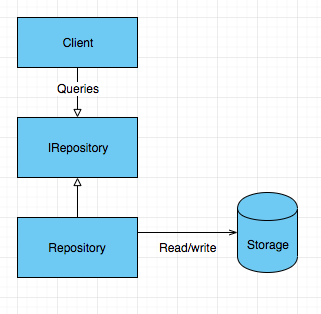
\includegraphics[scale=0.7]{grafiken/repositoryPattern.png}
    \caption{Repository Pattern overview}
    \label{fig:repositoryPattern}
\end{figure}


\begin{figure}[H]
    \centering 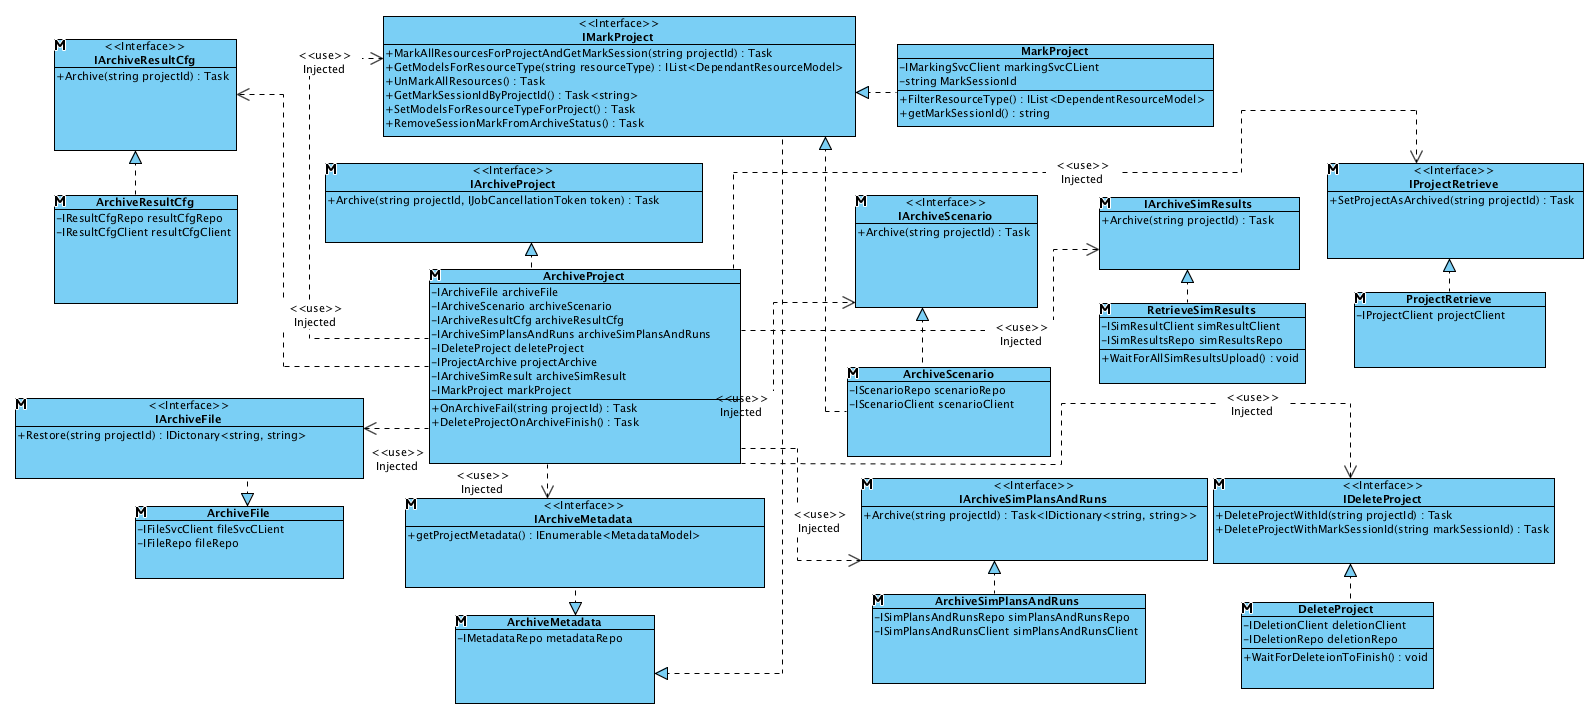
\includegraphics[height=6.5cm, angle=90, origin=c, width=11cm]{grafiken/archiveClass.png}
    \caption{Class Diagram for the Archive process (Top level)}
    \label{fig:archiveClassDiagram}
\end{figure}

\subsection{Challenges}
%There were couple of issues faced during the implementation phase for the archive. 
%Firstly, this dump feature has to be integrated in the Database utility service, given that the service could handle multiple requests. It is a mandatory requirement that the Database
%utility service could process more than one job at once. Therefore, an endpoint was needed which could be called by the archive service for multiple Mongo dump
%requests. To solve this problem, it is decided that the API requests would be executed as a long running job. 

A major issue to be discussed is when the archive process fails which requires a rollback by unmarking the project. As mentioned earlier the project is
marked as "TO\_BE\_ARCHIVED" so that no other processes can modify the contents during the archive process. This is a great strategy if everything goes as planned but 
often enough this is not the case and it is mandatory that an unmarking of the project is done otherwise the project would be unusable. It also happens that since the
marking service is dependent upon many services it has a very high rate of failure as well. This brings upon the problem how would the archive service behave if the
unmarking of the project fails. It seems very natural to just repeat the process until the unmarking request would succeed since it is absolutely necessary to unmark
a project. 
Translating this in terms of computer 
language an infinite loop until success. If this happens only with a single process it does not make a huge difference but thinking of the bigger picture if this 
occurs with 100 different processes at the same time, it would use valuable processing resources as it may be stuck in a deadlock condition until a outside interruption
is made. To avoid this condition of deadlock the number of retries for unmarking the project is restrained to a fixed number with certain time interval for the request 
calls. Currently it retries for at least a day and if it still fails the process would stop 
(See Listing \ref{lst:unmarkRetry}). 
Although, this solves the issue of using up resources but the problem that the project is unusable is still there. No other way except a manual unmarking is seen so 
it is decided that the archive process would also persist the marking session id which can be used to call the unmarking endpoint. With the use of this id a manual 
trigger is possible as soon as the error is fixed. The marking session id can be easily retrieved also from the GUI as it will be included in the status request of
the archive job.

\begin{lstlisting}[language={[Sharp]C}, caption={Unmarking retry implementation}, captionpos=b,label={lst:unmarkRetry}]
private async Task OnArchiveFail(string projectId)
{
    var timeInterval = 16;
    var restartCount = 0;
    var sessionId = await _iMarkProject.GetMarkSessionIdByProjectId(projectId);
    restartCount = 0;
    while (true)
    {
        try
        {
            Console.WriteLine($"Unmarking id {sessionId}");
            _iMarkProject.UnMarkAllResources(sessionId).Wait();
            await _iMarkProject.RemoveSessionMarkFromArchiveStatus(projectId);
            break;
        }
        catch (Exception e)
        {
            restartCount++;
            Console.WriteLine($"Unmarking restart {restartCount} and will start in {timeInterval}s");
            Task.Delay(TimeSpan.FromSeconds(timeInterval)).Wait();
            Console.WriteLine(e);
            if (restartCount == 5400) break;
        }
    }
}
\end{lstlisting}
